% This is based on the LLNCS.DEM the demonstration file of
% the LaTeX macro package from Springer-Verlag
% for Lecture Notes in Computer Science,
% version 2.4 for LaTeX2e as of 16. April 2010
%
% See http://www.springer.com/computer/lncs/lncs+authors?SGWID=0-40209-0-0-0
% for the full guidelines.
%
\documentclass{llncs}\usepackage[]{graphicx}\usepackage[]{color}
%% maxwidth is the original width if it is less than linewidth
%% otherwise use linewidth (to make sure the graphics do not exceed the margin)
\makeatletter
\def\maxwidth{ %
  \ifdim\Gin@nat@width>\linewidth
    \linewidth
  \else
    \Gin@nat@width
  \fi
}
\makeatother

\definecolor{fgcolor}{rgb}{0.345, 0.345, 0.345}
\newcommand{\hlnum}[1]{\textcolor[rgb]{0.686,0.059,0.569}{#1}}%
\newcommand{\hlstr}[1]{\textcolor[rgb]{0.192,0.494,0.8}{#1}}%
\newcommand{\hlcom}[1]{\textcolor[rgb]{0.678,0.584,0.686}{\textit{#1}}}%
\newcommand{\hlopt}[1]{\textcolor[rgb]{0,0,0}{#1}}%
\newcommand{\hlstd}[1]{\textcolor[rgb]{0.345,0.345,0.345}{#1}}%
\newcommand{\hlkwa}[1]{\textcolor[rgb]{0.161,0.373,0.58}{\textbf{#1}}}%
\newcommand{\hlkwb}[1]{\textcolor[rgb]{0.69,0.353,0.396}{#1}}%
\newcommand{\hlkwc}[1]{\textcolor[rgb]{0.333,0.667,0.333}{#1}}%
\newcommand{\hlkwd}[1]{\textcolor[rgb]{0.737,0.353,0.396}{\textbf{#1}}}%

\usepackage{framed}
\makeatletter
\newenvironment{kframe}{%
 \def\at@end@of@kframe{}%
 \ifinner\ifhmode%
  \def\at@end@of@kframe{\end{minipage}}%
  \begin{minipage}{\columnwidth}%
 \fi\fi%
 \def\FrameCommand##1{\hskip\@totalleftmargin \hskip-\fboxsep
 \colorbox{shadecolor}{##1}\hskip-\fboxsep
     % There is no \\@totalrightmargin, so:
     \hskip-\linewidth \hskip-\@totalleftmargin \hskip\columnwidth}%
 \MakeFramed {\advance\hsize-\width
   \@totalleftmargin\z@ \linewidth\hsize
   \@setminipage}}%
 {\par\unskip\endMakeFramed%
 \at@end@of@kframe}
\makeatother

\definecolor{shadecolor}{rgb}{.97, .97, .97}
\definecolor{messagecolor}{rgb}{0, 0, 0}
\definecolor{warningcolor}{rgb}{1, 0, 1}
\definecolor{errorcolor}{rgb}{1, 0, 0}
\newenvironment{knitrout}{}{} % an empty environment to be redefined in TeX

\usepackage{alltt}
\usepackage{listings}
\usepackage{moreverb}
\IfFileExists{upquote.sty}{\usepackage{upquote}}{}
\begin{document}
\title{Stat243 : Problem Set 1}
%                                     also used for the TOC unless
%                                     \toctitle is used
%
\author{Thibault Doutre}
%
%%%% list of authors for the TOC (use if author list has to be modified)
%
\institute{September 11, 2015}

\maketitle              % typeset the title of the contribution
Sometimes, I had to split lines of code. Be sure to copy line after line before pasting it into the bash shell. 


%%%%%%%%%%%%%%%%%%%%%%%%%%%%%%%%%%%%%%%%%%%%%%%%%%%%%%%%%%%
\section{Problem 1}
%%%%%%%%%%%%%%%%%%%%%%
\subsection{Part a}
Load the data into a tar.gz file using wget.
\begin{lstlisting}[frame=single] 
wget -O test.tar.gz "http://data.un.org/Handlers/Download
Handler.ashxDataFilter=itemCode:526&DataMartId=FAO&Format
=csv&c=2,3,4,5,6,7&s=countryName:asc,elementCode:asc,year
:desc" 
\end{lstlisting}
Decompress the data and rename it.
\begin{lstlisting}[frame=single] 
tar -zvxf test.tar.gz 
mv UNdata_Export_20150902_002111523.csv apricots.csv
\end{lstlisting}
Regions of the world have a "+" at the end of their names. In order to make the distinction between them and single countries is : \\ 
Select lines containing + and put them into a file while displaying the content of the file using tee. 
\begin{lstlisting}[frame=single] 
grep .+ apricots.csv | tee data_areas.txt
\end{lstlisting}
Select lines without + using the -v flag | remove the last 7 lines containing the legend | remove the first line which is useless | use tee command to put this into a file and display it
\begin{lstlisting}[frame=single] 
grep -v .+ apricots.csv | ghead -n -7 | sed '1d' | tee dat
a_countries.txt
\end{lstlisting}
Subset data according to year 2005 using awk. Make a condition over the 4th colum of the data.
\begin{lstlisting}[frame=single] 
awk -F'[,]' '$4~"2005"' data_countries.txt
\end{lstlisting}
Select a subset of data corresponding to the year 2005 | select lines containing "Area Harvested" | remove quotation marks in all the data | sort by numerical value the 6th column (decreasing) | select the top 5 countries | only display names 
\begin{lstlisting}[frame=single]  % Start your code-block

awk -F'[,]' '$4~"2005"' data_countries.txt | grep "Area 
Harvested" | sed 's/\\"//g' | sort -t"," -k6 -n -r | head 
-n 5 | cut -d',' -f1
\end{lstlisting}
Creating script with vim editor
\begin{lstlisting}[frame=single] 
vim scriptA.sh
\end{lstlisting}
Content of the script :
\begin{itemize}
\item For every year listed below, display it then display the top five countries found as described above.
\end{itemize}
\begin{boxedverbatim}
for i in 1965 1975 1985 1995 2005
do
        echo $i
        echo $(awk -F'[,]' '$4~'$i'' data_countries.txt |
		grep "Area Harvested" | sed 's/\\"//g' | sort -t"," -k6 
-n -r | head -n 5 | cut -d',' -f1)
done 
\end{boxedverbatim}


Execute the script with the bash command.
\begin{lstlisting}[frame=single] 
bash scriptA.sh
\end{lstlisting}
Here are the rankings for the years 1965, 1975, 1985, 1995 and 2005 :\\\\
1965 - USSR Turkey United States of America Spain Tunisia\\
1975 - USSR Turkey Spain Tunisia Italy\\
1985 - Turkey USSR Spain Tunisia Italy\\
1995 - Turkey Spain Ukraine Tunisia Russian Federation\\
2005 - Turkey Pakistan Uzbekistan Algeria Spain
\subsection{Part b}
Creating the script
\begin{lstlisting}[frame=single] 
vim Bscript.sh
\end{lstlisting}
Content of the script :
\begin{itemize}
\item Download the file with wget and put it into a tar.gz file
\item Decompress the file
\item Get the name of the file and display it on the screen
\item Delete both files in order to avoid keeping every single file. \item This ensure that there is only one file beginning with "UNdata". It is convenient for the grep command. 
\end{itemize}
\begin{boxedverbatim}
#!/bin/bash
function foo1
{
wget -O test0.tar.gz "http://data.un.org/Handlers/Download
Handler.ashxDataFilter=itemCode:$1&DataMartId=FAO&Format=c
sv&c=2,3,4,5,6,7&s=countryName:asc,elementCode:asc,year:de
sc"

tar -zxvf  test0.tar.gz

ls UNdata_* | xargs cat

ls UNdata_* | xargs rm

rm test0.tar.gz
} 
\end{boxedverbatim}

Display avocados.csv from the script for example (572)
\begin{lstlisting}[frame=single]
source Bscript.sh ; foo1 572 
\end{lstlisting}
\subsection{Part c}
Open script
\begin{lstlisting}[frame=single] 
vim Dscript.sh
\end{lstlisting}
Content of the Script :
\begin{itemize}
\item Download the meta data from the FAO website.
\item Grep for the only line who matters here i.e. the one containing the correspondence between numbers and the names of the files.
\item Delete everything after the keyword because it is useless.
\item Take the 3 last characters using tail.
\item Then, call foo1 function from Bscript.sh and run it with the good corresponding number.
\end{itemize}
\begin{boxedverbatim}
#!/bin/bash

getData(){


local locvar=$(curl "http://data.fao.org/dimension-member?
entryId=8462e2d6-ba52-492c-a0a7-e08893a59aac" | grep ">Def
ault composition" | sed -n -e 's/ '$1'.*//p' | tail -c 
4)

source Bscript.sh
foo1 $locvar > $1.txt
}
\end{boxedverbatim}

Run the function getData() with Avocados as an example
\begin{lstlisting}[frame=single]
source Dscript.sh ; getData Avocados
\end{lstlisting}
%%%%%%%%%%%%%%%%%%%%%%%%%%%%%%%%%%%%%%%%%%%%%%%%%%%%%%%%%%%%%
\section{Problem 2}
Create the script
\begin{lstlisting}[frame=single] 
vim Cscript.sh
\end{lstlisting}
Content of the script :\\\\
How to get names of the files :
\begin{itemize}
\item Download URL 
\item Look for text files
\item Remove part before "href="
\item Remove part after ".txt"
\end{itemize}
How to download them :
\begin{itemize}
\item For every name of the text files we want to download, download it by adding the name at the end of the corresponding URL.
\item Display message which shows the name of the file
\end{itemize}


\begin{boxedverbatim}
#!/bin/bash
for a in $(curl http://www1.ncdc.noaa.gov/pub/data/ghcn/
daily/ | grep .'\.txt' | sed -n -e 's/.*href=\" *//p' | s
ed -n -e 's/\">.*//p')
do

curl -o $a "http://www1.ncdc.noaa.gov/pub/data/ghcn/daily
/"$a

echo "Download [file :\ "$a"] in progress..."
done 
\end{lstlisting}
Run script
\begin{lstlisting}[frame=single]
bash Cscript.sh 
\end{boxedverbatim}
\section{Problem 3}
The height of the water level in Lake Huron fluctuates over time. Here I ’analyze’ the variation using R. I show a histogram of the lake levels for the period 1875 to 1972.
\begin{knitrout}
\definecolor{shadecolor}{rgb}{0.969, 0.969, 0.969}\color{fgcolor}\begin{kframe}
\begin{alltt}
\hlkwd{hist}\hlstd{(LakeHuron)}
\end{alltt}
\end{kframe}
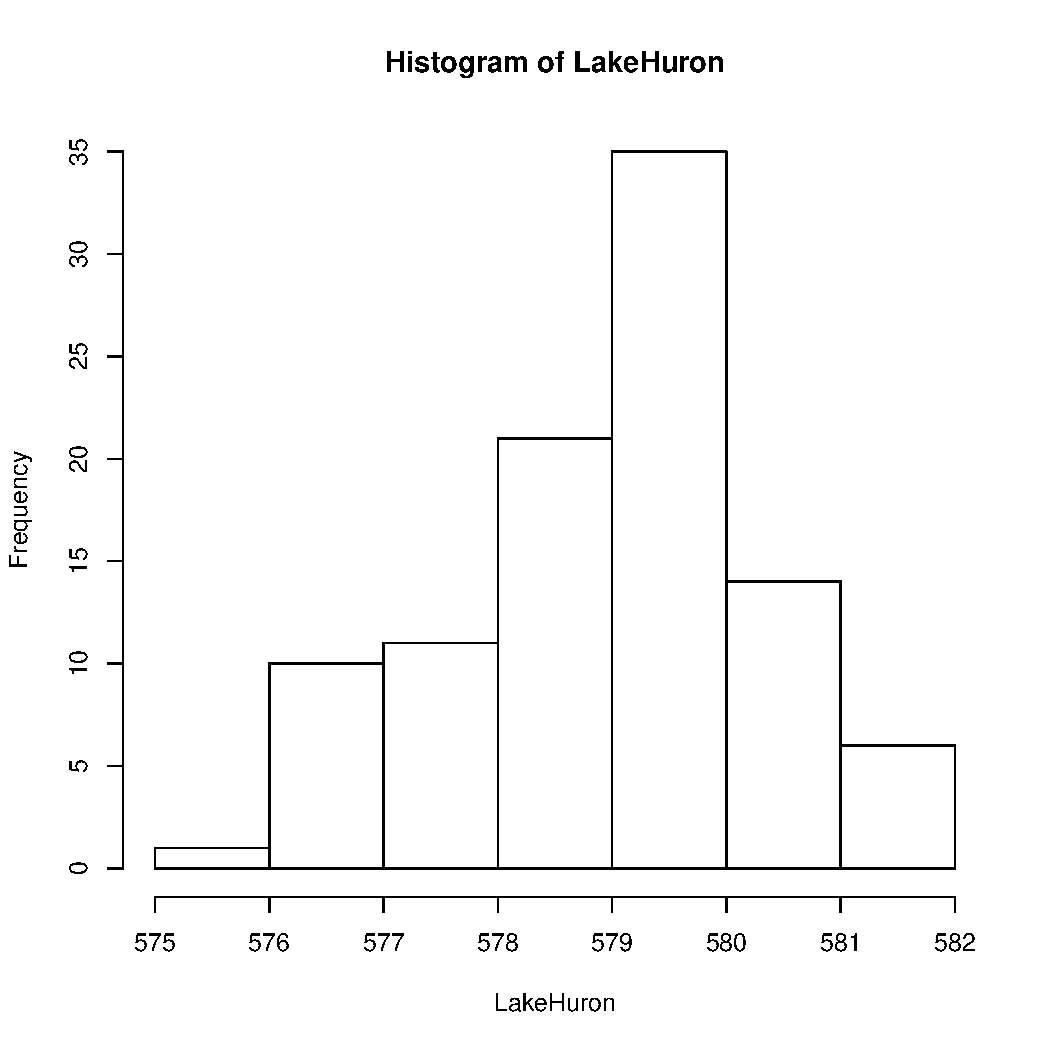
\includegraphics[width=\maxwidth]{figure/__-1} 
\begin{kframe}\begin{alltt}
\hlstd{lowHi} \hlkwb{<-} \hlkwd{c}\hlstd{(}\hlkwd{which.min}\hlstd{(LakeHuron),} \hlkwd{which.max}\hlstd{(LakeHuron))}
\hlstd{yearExtrema} \hlkwb{<-} \hlkwd{attributes}\hlstd{(LakeHuron)}\hlopt{$}\hlstd{tsp[}\hlnum{1}\hlstd{]}\hlopt{-}\hlnum{1} \hlopt{+} \hlstd{lowHi}
\end{alltt}
\end{kframe}
\end{knitrout}
\end{document}
